\subsection{Pretraining Data}
\label{sec:pretrain_data}

In this sub-section, we describe new datasets that we added to our pretraining corpus since Nemotron Nano 2. We are releasing the vast majority of the new data on HuggingFace,
%\todo{Markus Kliegl: add link to collection}
divided into four main datasets. We describe each of these in more detail below.
% Note: Based on customer feedback, the goal is to group & name things similar to
% how we release on HuggingFace, so it's easier to match up what's in the tech report with
% what's in the released datasets.
%
% We may not literally keep these subsubsection names.
% We may have to reorganize a bit if we can't release some of the data described.


\subsubsection{Nemotron-CC-Code-v1}

We first filtered out the code pages in Common Crawl based on a fast pattern matching code classifier for webpages. We then constructed our high-quality code pretraining corpus by applying a modified version of the Nemotron-CC-Math pipeline~\citep{karimi2025nemotronccmath} to Common Crawl pages containing code. 

Starting from raw HTML, we rendered each document using Lynx, which reliably preserved code layout, indentation, and inline technical elements. The resulting text was processed by an LLM-based cleaning stage using the Phi-4 model, which removed boilerplate while strictly retaining code snippets, configuration blocks, API references, and mathematical expressions. To ensure that only programming-relevant documents are included, we applied a lightweight code-quality relevance classifier, filtering out non-technical pages and retaining documents with substantial or complete code content. This pipeline produced a 427.92B-token corpus in which equations are standardized to LaTeX, code blocks are preserved with structural fidelity, and noise is minimized. Compared to previous extraction approaches that often corrupt or truncate code examples, our method reliably recovered complete code snippets and technical context at scale. % guided by our HTML_TO_TEXT_PROMPT_CODE based on our CODE_QUALITY_PROMPT_SIMPLIFIED


\subsubsection{Nemotron-Pretraining-Code-v2}
We sourced additional code from GitHub for repositories we identified as missing from our existing corpus in addition to collecting recent data with a cut-off date of April 15, 2025. We used the same pipeline as described in ~\cite{nemotronnanov2} to curate the data and we remove exact and near-duplicate files already present in our existing corpus.

In addition to our raw source-code corpus, we synthetically generated additional mixed natural-language and source code documents using the Qwen3 32B LLM. Similar to our approach described in ~\cite{nvidia2025nemotronhfamilyaccurateefficient}, we prompted the model to generate question and answer pairs using our new source-code data as seeds. Additionally, we prompted the model to generate student-teacher (Python only) and code-review (Python/C++) style dialogue grounded with a combination of code snippets and full source files.

Following the code-rewriting work presented in ~\cite{fujii2025rewriting}, we also found that using LLMs to rephrase source code improved downstream code-generation accuracies. Using Qwen3 32B, we rephrased all of our raw Python source code using a combination of the Style-Guided Code Rewriting (SGCR) and Self-Contained Optimization Rewriting (SCOR) prompts ~\citep{fujii2025rewriting}, as well as our own prompt with similar intent. To ensure high-quality LLM rephrasing, as a post-processing step, we checked for syntax errors and assessed code-quality improvements using the Pylint Python linter for each of the rewritten files.

While LLM-based source-code rewriting can be observed as a transformation of the original source-code to an improved version, we extended this concept and applied it to source-code files from one language to another (i.e., code transpilation). Using Qwen3 32B we found that C++ tokens produced from Python using this transpilation procedure improved downstream C++ code-generation accuracy and thus served as a useful augmentation to our C++ subset. We applied this Python to C++ transpilation procedure to all Python source files in our source-code corpus.


\subsubsection{Nemotron-CC-v2.1}
% Markus Kliegl: Crawl refresh
For general English web crawl data, we added three more recent Common Crawl snapshots on top of \href{Nemotron-CC-v2}{https://huggingface.co/datasets/nvidia/Nemotron-CC-v2} (CC-MAIN-2025-18, CC-MAIN-2025-21, CC-MAIN-2025-26), prepared with the same Nemotron-CC recipe~\citep{su2024nemotroncctransformingcommoncrawl}. For all of the synthetic rephrasing, we used Qwen3-30B-A3B~\citep{yang2025qwen3technicalreport}. Just as for Nemotron Nano 2, we trained only on the Medium-Quality, Medium-High-Quality, and High-Quality buckets.

% Ying Lin
% \todo{Ying Lin: more synthetic crawl data (CC18)}
Previously, we rephrased only the High-Quality subset of Common Crawl data.
To further expand our corpus of unique high-quality tokens, we applied five prompts~\citep{su2024nemotroncctransformingcommoncrawl} to the Medium-High-Quality data from 110 Common Crawl snapshots (CC-MAIN-2013-20 - CC-MAIN-2025-26), resulting in 2.1T new tokens.

% Ying Lin
% \todo{Ying Lin, Dan Su: translated-to-English crawl data + quality classification + SDG}
Finally, we employed a new strategy to source high-quality English tokens by translating to English from other languages using Qwen3-30B-A3B. % Ying: I deleted the citation here as Qwen 3 tech report has been cited
We first translated documents from the latest three Common Crawl snapshots available at that time (CC-MAIN-2024-51, CC-MAIN-2025-08, and CC-MAIN-2025-18) in 9 languages (Chinese, French, German, Italian, Japanese, Polish, Portuguese, Russian, Spanish) to English.
% Specifically, for , we first translated from 9 languages (Chinese, French, German, Italian, Japanese, Polish, Portuguese, Russian, Spanish) to English.
After that, we applied the Nemotron-CC ensemble of quality classifiers to retain only High-Quality and Medium-High-Quality documents from this translated subset.
Additionally, we applied four of the five Nemotron-CC rephrasing prompts to the high-quality data to generate more unique tokens.
After training of \ourbasemodel was already underway, we found that some uninformative translated documents (e.g., daily conversations, ads) were receiving high scores from the Nemotron-CC quality classifiers.
To address this, for the released version of this dataset, we performed one additional pass of LLM-based quality filtering that removed approximately 10.6~\% of tokens, which slightly improved accuracies across benchmarks in an internal ablation.

Overall, we curated or generated over 2.5T new tokens from Common Crawl data.
%and are releasing this as \href{Nemotron-CC-v2.1}{https://huggingface.co/datasets/nvidia/Nemotron-CC-v2.1}.

\subsubsection{Nemotron-Pretraining-Specialized-v1}

This dataset comprises various synthetic datasets that are specialized for specific topics like STEM Reasoning or scientific coding. We describe the subsets in more detail below.

% Ying Lin
\newparagraph{Synthetic Wikipedia Data} We revised English Wikipedia articles using Qwen3-30B-A3B-Instruct-2507 to improve clarity and formatting. We discarded disambiguation and redirect pages and removed References, See also, Notes, and External Links sections. We also instructed the model to remove any irrelevant content such as uncleaned HTML elements.

% Ying Lin
\newparagraph{Synthetic Math Textbook Data}
We generated well-structured educational textbook-style sections from Nemotron-CC-Math~\citep{karimi2025nemotronccmath}.
We evaluated the mathematical content in each document and classify it into an educational level (e.g., grade school, middle school, high school) based on multiple factors such as involved mathematical concepts and complexity.
We kept documents containing mathematical content at the undergraduate level and above and developed each into a textbook-style section with diverse educational features such as definitions and illustrative examples.

% Ying Lin
\newparagraph{Synthetic Scientific Coding Data} Using STEM-related documents retrieved from Nemotron-CC as the seed data, we synthesized two types of documents:
(1) Code-embedded article: A comprehensive, in-depth, and well-formatted article that explores and implements a non-trivial, graduate- or research-level scientific or mathematical algorithm in Python;
(2) Computational coding problem: An advanced, computational, graduate- or research-level coding problem with Python solution. The main problem is decomposed into 5 to 15 logically ordered non-trivial substeps, each solved by an individual function. We extract the main problem, dependencies, substep descriptions, and each function's signature, docstring, body, and return statement and exclude examples where any of these components are missing.

\newparagraph{Synthetic Cross-Domain Code Data}
To generate more diverse and complex code data, we develop a novel approach we call \textit{InfiniByte} that cross-breeds multiple datasets together. When applied to code, InfiniByte creates entirely new programming problems by bringing together concepts from different fields to pose never before seen questions. In doing so, InfiniByte fills the problem space between disparate domains, generates questions at the boundary of model capabilities, and mimics how science is often advanced at the intersection of two or more fields.

Starting with a curated list of competitive coding problems from our groundbreaking OpenCodeReasoning dataset (\cite{ahmad2025opencodereasoning}), we systematically inject concepts from datasets across mathematics (OpenMathReasoning, \cite{moshkov2025aimo2}), physics (Physics Big, \cite{physics_big}), chemistry (IChO, \cite{icho_ipho}), and other sciences. We generate multiple problem candidates per (problem, concept) combination, select the best problem candidate, based on LLM-as-critic rubric that tests for clarity, difficulty, and adherence to the employed cross-breeding strategy. We then generate solutions to each new coding problem using a reasoning model such as \texttt{Qwen3-235B-A22B-Thinking-2507} \citep{yang2025qwen3technicalreport}. We cross-breed with two different strategies in mind:
\begin{enumerate}
    \item[1.] Obfuscate without really changing the original problem (this is common in competitive coding problems and other competitions).
    \item[2.] Complicate by actually making the new problem much more complex: the resulting problem is more challenging as it requires reasoning across multiple concepts to solve it. 
\end{enumerate}

The InfiniByte data generation pipeline was implemented in NeMo Data Designer (\cite{nemo-data-designer}), NVIDIA’s state-of-the-art synthetic data generation framework. This allowed our complex pipeline to benefit from the compound AI approach of the framework in order to enforce proper concept grounding via Jinja templating, guarantee structured outputs required at all stages, incorporate feedback loops, as well as perform data validation and automated retries. 

\newparagraph{Synthetic STEM Reasoning}
To reinforce complex reasoning capabilities within STEM domains, we built the Reasoning Question-Answer (RQA) dataset. Our goal in the creation of RQA was two-fold: 
%
\begin{enumerate}
    \item[i)] Demonstrate advanced scientific reasoning and instruction following that can be further reinforced in post-training, as shown in \cite{akter2025frontload}.
    \item[ii)] Reinforce correlations between advanced topics that are otherwise rarely observed in web-scale data. 
\end{enumerate}
%
The dataset was generated in four steps. First, we targeted diverse and advanced scientific texts as seed data. Starting from the STEM subset of the Essential-Web web-scale dataset \citep{essentialweb}, we filtered the dataset using the Essential-Web taxonomy to documents that met the following criteria:
%
\begin{itemize}
    \item Undergraduate or graduate education level.
    \item No extraction artifacts, no missing content.
    \item Advanced reasoning depth.
    \item High or exceptional technical correctness.
    \item Leverages one of the Bloom cognitive processes: \emph{Analyze}, \emph{Evaluate} or \emph{Create}.
    \item Leverages one of the Bloom knowledge domains: \emph{Conceptual}, \emph{Procedural} or \emph{Metacognitive}.
    \item In the English language and over 1000 characters.
\end{itemize}

This filtering resulted in approximately 14 million documents. Next, we used hierarchically stratified sampling on document topics to trade-off between seed document volume and diversity. Leveraging the Free Decimal Correspondence (FDC) numerical topic code from the Essential-Web taxonomy, documents were ordered in hierarchical round-robin fashion across multiple orders of magnitude in the FDC code, from high-level topic domains (e.g. Physics, Chemistry, Math, Computer Science) to lower-level subdomains (e.g. Thermodynamics, Quantum Mechanics). Using this approach, we could apply any cutoff N to the seed documents to ensure maximum diversity for a given volume of documents; while we generated RQA samples for the first 9 million samples, we ultimately chose to use the first 4.5 million for training. To limit the length of each seed document, we post-processed documents over 4096 characters in length to extract a random contiguous text chunk consisting of <4096 characters.

Each seed document was presented as context to \texttt{Qwen3-235B-A22B-Thinking-2507}, which was prompted to use the STEM content as inspiration for a difficult (yet answerable) graduate-level scientific reasoning question. The model was instructed to ensure that the question did not require access to the original seed passage to answer. Examples were discarded if they failed to produce a question within 8192 reasoning tokens.

Finally, this question was presented to \texttt{Qwen3-235B-A22B-Thinking-2507} to answer in a second generation step, without including the seed passage as context. The resulting reasoning trace and answer were filtered to remove model-specific idiosyncrasies, limited to 8192 characters, and concatenated with the question to produce a single RQA example. The two-step generation process was designed to maximally engage the teacher model's reasoning capabilities, both in generating a difficult question from the seed document and in answering its own question. The resulting pretraining dataset consists of 4.3 million RQA demonstrations for a total of approximately 31.7 billion unique tokens. 

To make further use of the stratified STEM seed documents, we also produced a diverse QA (DQA) version of the dataset, using the first 9 million seed documents in stratification order for a total of approximately 8 billion tokens. The STEM DQA dataset was built by using the DQA prompt \& generation procedure as demonstrated in Nemotron-CC \citep{su2024nemotroncctransformingcommoncrawl}, which concatenates a contiguous text chunk from the source document with short-form question-answer pairs. We utilized \texttt{Qwen3-30B-A3B} to generate these QA pairs.

Both RQA and DQA data generation pipelines were implemented in NeMo Data Designer (\cite{nemo-data-designer}).

%\todo{Markus Kliegl: brief description of or pointers to the new post-training SFT datasets included in pre-training}
\newparagraph{SFT-style data.}
We included new and refreshed SFT datasets in pretraining for code, math, and STEM, just as for Nemotron Nano 2. Detailed synthesis methods and pipelines can be found in prior works~\citep{toshniwal2024openmathinstruct, moshkov2025aimo2,bercovich2025llamanemotronefficientreasoningmodels,ahmad2025opencodereasoning,ahmad2025opencodeinstruct,majumdar2024genetic}.
% STEM-SFT: See Section 3.1.3 of Llama-Nemotron paper - https://arxiv.org/abs/2505.00949v1
% \todo{Wasi Uddin Ahmad: cite OCR 1 and 2, SWE Zero (if arxiv will be out by then)}
% \todo{Zihan Liu: code and math SFT data}
We also incorporated a set of additional math and code SFT samples from AceReason-Nemotron-1.1~\citep{liu2025acereason}. This collection encompasses a wide range of prompt sources, including NuminaMath~\citep{numina_math_datasets}, OrcaMathWordProblems~\citep{mitra2024orca}, MathInstruct~\citep{yue2023mammoth}, and MetaMathQA~\citep{yu2023metamath} for math tasks, as well as TACO~\citep{li2023taco}, APPs~\citep{hendrycksapps2021}, OpenCoder-Stage2~\citep{Huang2024OpenCoderTO}, and OpenCodeReasoning~\citep{ahmad2025opencodereasoning} for coding tasks. The responses for these prompts are generated by DeepSeek-R1~\citep{deepseekai2025deepseekr1incentivizingreasoningcapability}.


\subsection{Data Mixture and Ordering}
\label{section:blend}

Our pretraining corpus spans fifteen data categories.
The largest component is web crawl data, which we subdivide into five quality-based groups following the Nemotron-CC taxonomy~\citep{su2024nemotroncctransformingcommoncrawl}: crawl-medium, crawl-medium-high, syn-crawl-medium-high, crawl-high, and syn-crawl-high, representing medium, medium-high, high,  crawl data.
Beyond web crawl, the mixture also includes math, Wikipedia, code, nemotron-cc-code, academic text, Crawl$++$, multilingual data, and synthetic SFT-style datasets, the latter further grouped into general-sft, stem-sft, and code-sft categories.
Crawl$++$ comprises the OpenWebText, BigScience and Reddit datasets. 
Our multilingual data has nineteen languages:
Arabic, Chinese, Czech, Danish, Dutch, Finnish, French, German, Hebrew, Hindi, Italian, Japanese, Korean, Portuguese, Polish, Russian, Spanish, Swedish, and Thai. 
We design our data mixtures to balance coverage and quality by assigning comparable weight to sources of similar estimated quality. Higher-quality datasets are prioritized accordingly, receiving greater weight in the blend. Additional details on our dataset quality assessment and mixture construction methodology can be found in \cite{feng2024maximizedataspotentialenhancing} and \cite{nvidia2025nemotronhfamilyaccurateefficient}.


We used a curriculum based on two phases to pre-train \ourbasemodel. 
In the first phase, we used a data mixture that promotes diversity in data; in the second phase, we primarily use high-quality datasets (e.g., Wikipedia). 
We switched to the second phase at the 94\% point of training. 
The data mixtures used in each phase are shown in Figure~\ref{fig:phase-blends}. 

\begin{figure}[htbp]
    \centering
    \begin{subfigure}{0.49\textwidth}
        \centering
        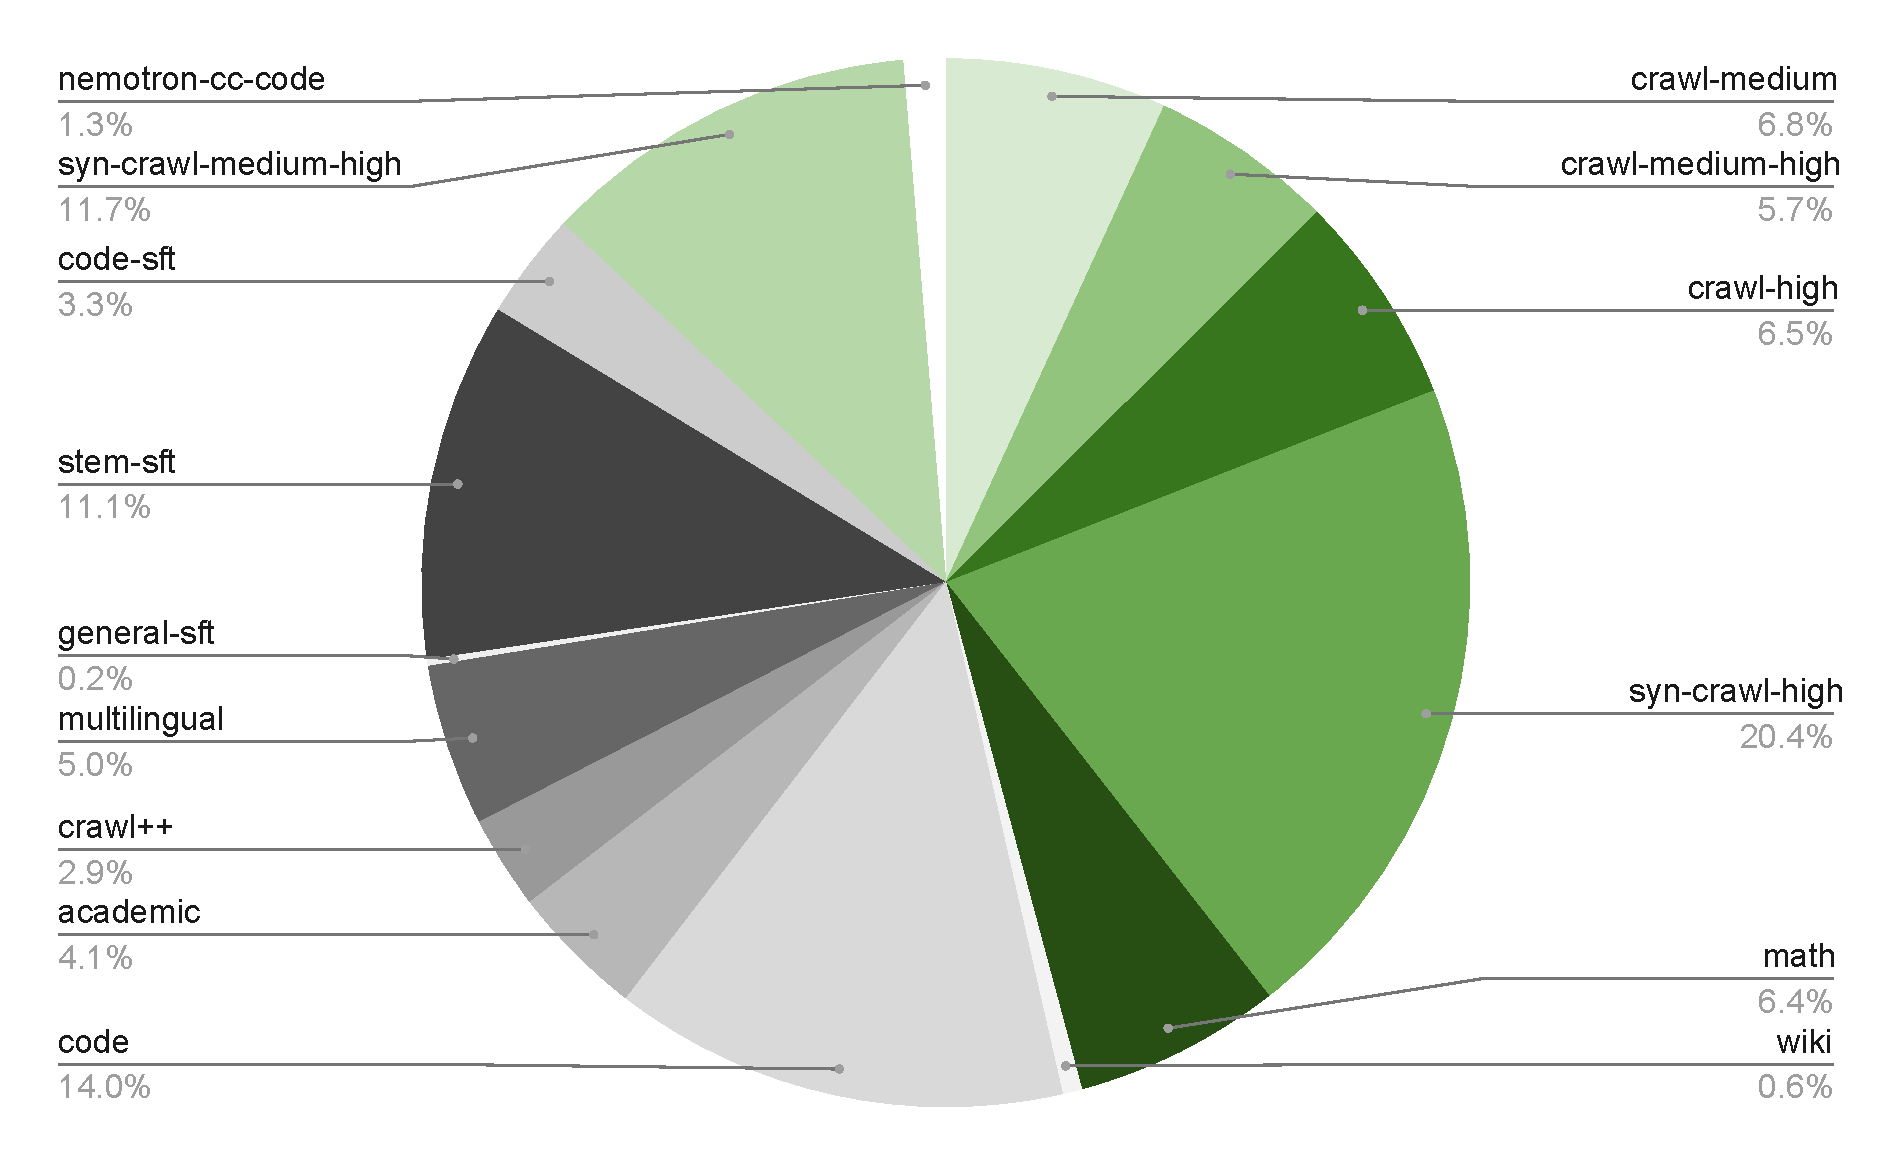
\includegraphics[width=\linewidth]{figures/nanov3_phase1_blend.pdf}
        \caption{Data mixture of Phase 1.}
        \label{fig:phase1-blend}
    \end{subfigure}
    \begin{subfigure}{0.49\textwidth}
        \centering
        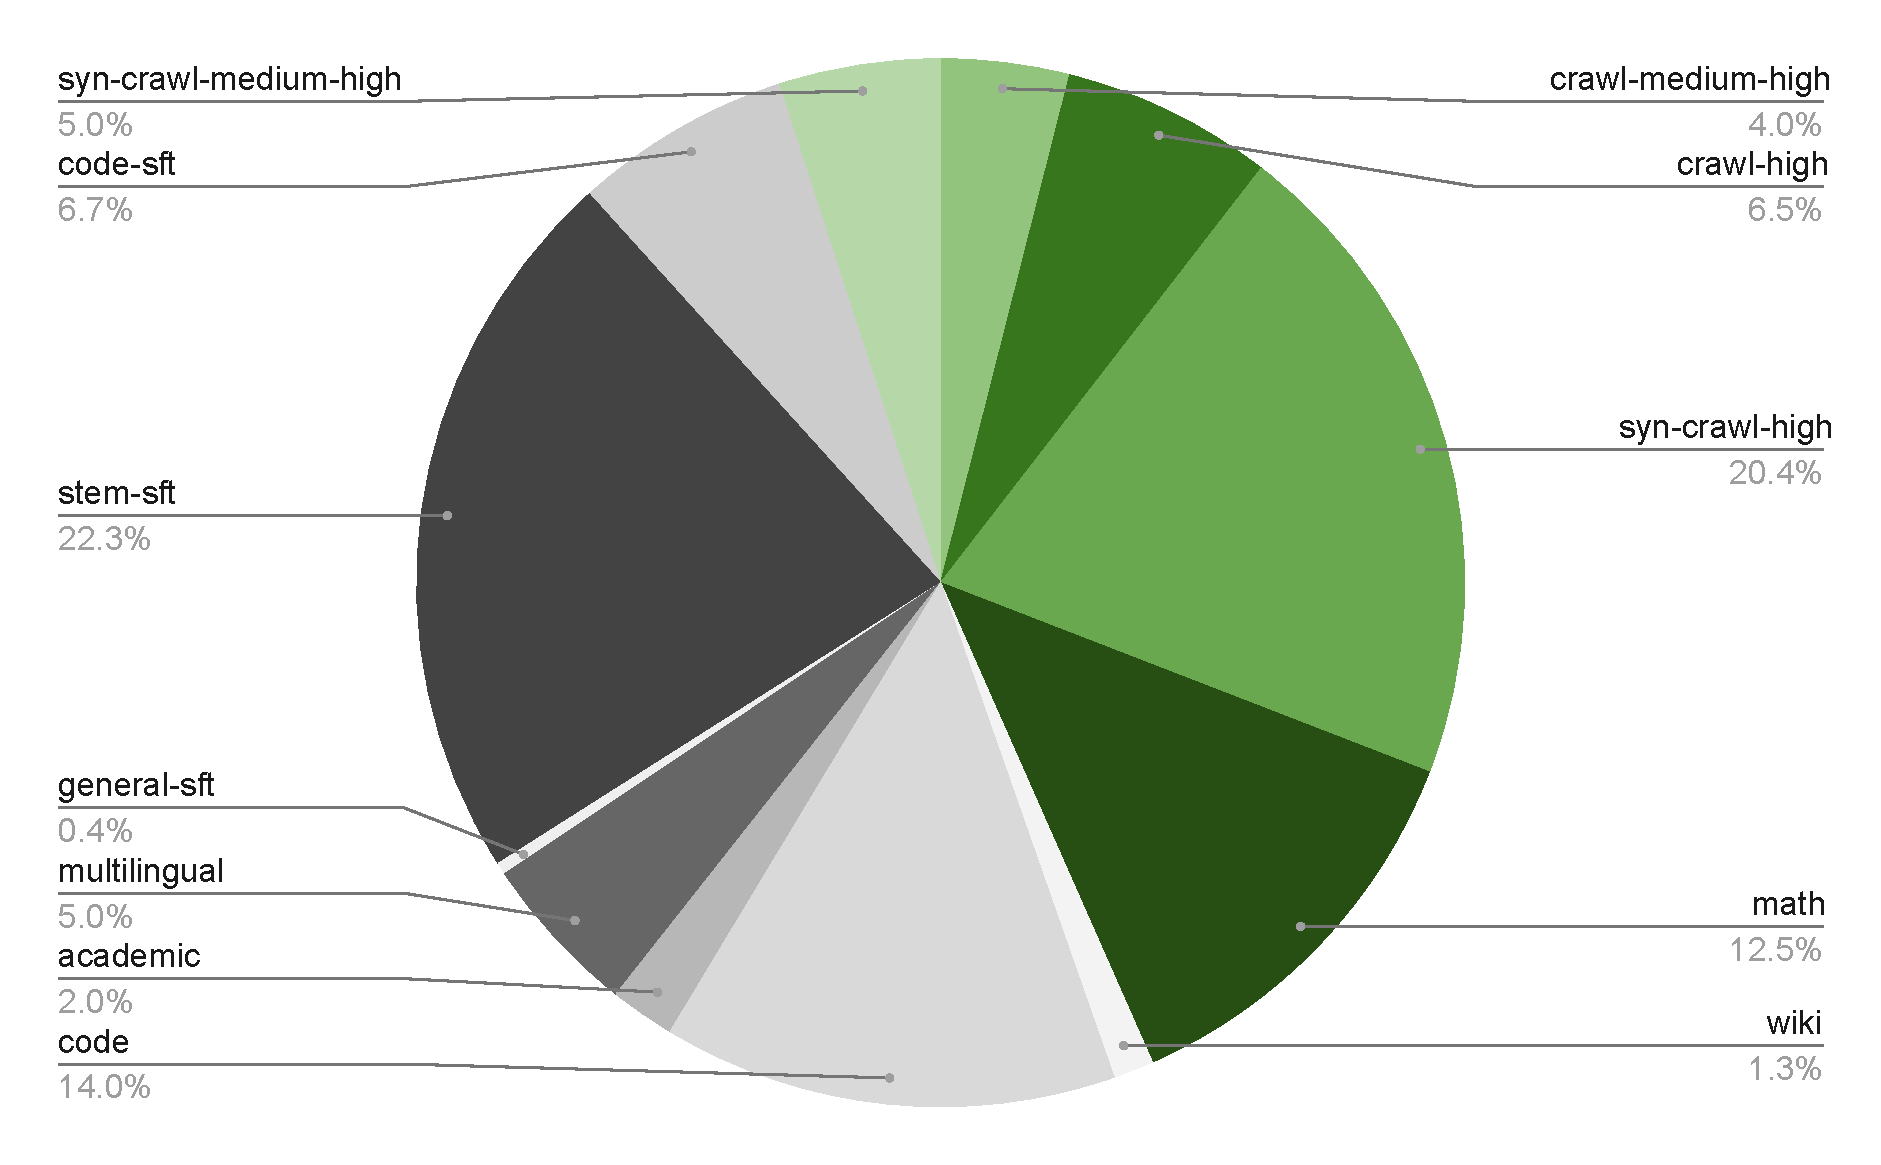
\includegraphics[width=\linewidth]{figures/nanov3_phase2_blend.pdf}
        \caption{Data mixture of Phase 2.}
        \label{fig:phase2-blend}
    \end{subfigure}
    \caption{Data mixtures for each phase of pre-training.}
    \label{fig:phase-blends}
\end{figure}


% \todo{Shrimai Prabhumoye, Abhinav Khattar, John Kamalu}
